\section{Far-Field Radiation}
Last time, we wrote down the expression for the electromagnetic fields generated by a moving charge with trajectory $\v{r}(t)$:

\begin{equation}
    \v{E}(t, \v{x}) = q\frac{\mu_0 c^2}{4\pi}\frac{(\hat{\v{n}} - \frac{1}{c}\dod{\v{r}}{t})(1 - \frac{1}{c^2}\left(\dod{\v{r}}{t}\right)^2)}{\alpha^3\abs{\v{x} - \v{r}(t_{\text{ret}})}^2} + q\frac{\mu_0}{4\pi}\frac{\hat{\v{n}} \times [(\hat{\v{n}} - \frac{1}{c}\dod{\v{r}}{t})\times \dod[2]{\v{r}}{t}]}{\alpha^3\abs{\v{x} - \v{r}(t_{\text{ret}})}}
\end{equation}
\begin{equation}
    c\v{B}(t, \v{x}) = \hat{\v{n}} \times \v{E}(t, \v{x})
\end{equation}
with:
\begin{equation}
    \alpha = \abs{-\frac{1}{c}\hat{\v{n}}\cdot\dod{\v{r}}{t}(t_{\text{ret}})}, \quad \hat{\v{n}} = \frac{\v{x} - \v{r}(t_{\text{ret}})}{\abs{\v{x} - \v{r}(t_{\text{ret}})}}, \quad t_{\text{ret}} = t - \frac{1}{c}\abs{\v{x} - \v{r}(t_{\text{ret}})}
\end{equation}

\subsection{Poynting Vector and Power}
The reason why this all looks so complicated is that this is the exact result that applies to all cases. You can check that for $\v{r}(t) = \v{x}_0$ that this reduced to the Coloumb field. If $\v{x}(t) = \v{x}_0 + vt$, this reduces to a problem you had in your second problem set (which you can solve via boost). If you were only interested in these two cases, it would be madness to calculate the general case and restrict after, but we are interested in slightly more sophisticated scenarios. In particular, we want to study radiation. As you learned in the last quarter, the hero of the story is the Poynting vector:
\begin{equation}
    \v{S} = \frac{1}{\mu_0}\v{E} \times \v{B}
\end{equation}

We are interested in looking at the radiation a large distance from the source, and hence the $\frac{1}{x^2}$ (with $x = \abs{\v{x} - \v{r}(t_{\text{ret}})} \approx \abs{\v{x}}$.

\begin{center}
    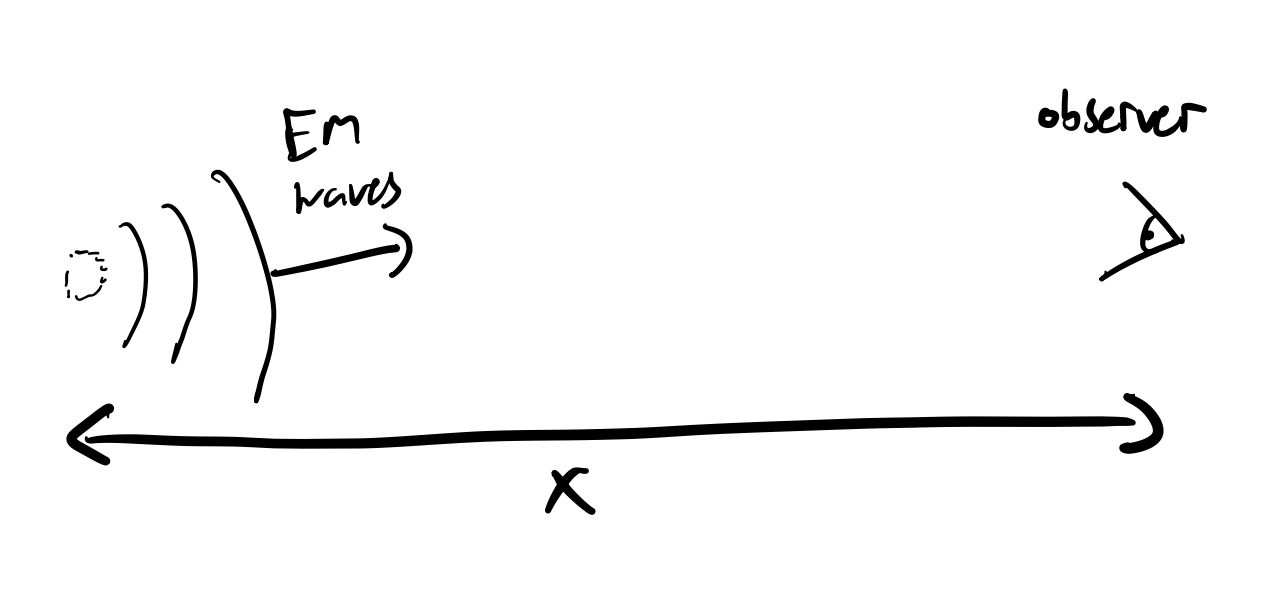
\includegraphics[scale=0.38]{Lectures/Images/lec9-farfield.png}
\end{center}

We take the particle motion to be approximately confined to the origin) contributions to $\v{S}$ (all higher order terms we will drop). Looking at $\v{E}/\v{B}$, we have two terms:
\begin{equation}
    \v{E} \sim \frac{1}{x^2} + \frac{1}{x}
\end{equation}
\begin{equation}
    \v{B} \sim \v{E} \sim \frac{1}{x^2} + \frac{1}{x}
\end{equation}
So when we calculate $\v{S}$ by taking their cross product, the leading contribution will come from the product of the two $\frac{1}{x}$ terms.

For a given solid angle $d\Omega$, what is the power (energy/time) $dP$ that goes into it? 

\begin{center}
    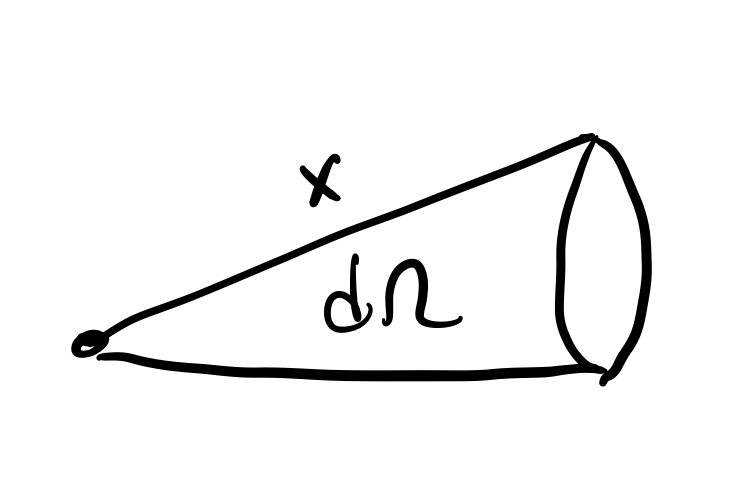
\includegraphics[scale=0.38]{Lectures/Images/lec9-solidangle.png}
\end{center}

Recall from last quarter that:
\begin{equation}
    \dod{P}{\Omega} = \lim_{\v{x} \to \infty}\abs{\v{x}}^2\v{S} \cdot \hat{\v{x}}
\end{equation}
Be aware that the $P$ above is not the same as the momentum density of the field:
\begin{equation}
    \v{P} = \e_0 \v{E} \times \v{B}
\end{equation}

For us, the power per solid angle is given (after only retaining terms of $\frac{1}{x^2}$):
\begin{equation}\label{eq:powerpersolidangle}
    \dod{P}{\Omega} = \frac{q^2\mu_0}{16\pi^2c\alpha^6}\abs{\hat{\v{x}}\times\left[\left(\hat{\v{x}} - \frac{1}{c}\dod{\v{r}}{t}\right) \times \dod[2]{\v{r}}{t}\right]}^2
\end{equation}
where the time derivatives are evaluated at $t_{\text{ret}}$, which reduces to:
\begin{equation}
    t_{\text{ret}} = t - \frac{1}{c}\abs{\v{x}}
\end{equation}
after taking $\v{x} \gg \v{r}$. Note from Eq. \eqref{eq:powerpersolidangle} that if we have no acceleration, then we have no radiation.

Note that we can write down a related quantity $\od{P'}{\Omega}$, with $P'$ the energy per unit retarded time (the energy seen by the emitter):
\begin{equation}
    \dod{P'}{\Omega} = \dod{P}{\Omega}\dod{t}{t_{\text{ret}}} = \dod{P}{\Omega} \alpha = \frac{q^2\mu_0}{16\pi^2c\alpha^5}\abs{\hat{\v{x}}\times\left[\left(\hat{\v{x}} - \frac{1}{c}\dod{\v{r}}{t}\right) \times \dod[2]{\v{r}}{t}\right]}^2
\end{equation}
In other words, if we know how to calculate one, we can easily obtain the other.

\subsection{Nonrelativistic Limit \& Connection to Dipoles}
Note that even though the particle is accelerating, we can put ourselves in a frame where $\od{\v{x}}{t} = \v{0}$ (more specifically, we can consider that the particle is moving sufficiently slowly that $\frac{1}{c}\od{\v{x}}{t} \ll 1$) instantaneously at $t_{\text{ret}}$. Then:
\begin{equation}
    \alpha = 1 - \frac{1}{c}\hat{\v{n}}\cdot\dod{\v{x}}{t}(t_{\text{ret}}) = 1
\end{equation}
In this case, we can write down a simpler looking formula:
\begin{equation}
    \left.\dod{P'}{\Omega}\right|_{\od{\v{x}}{t}=0} = \frac{q^2\mu_0}{16\pi^2c}\abs{\hat{\v{x}}\times\left[\hat{\v{x}} \times \dod[2]{\v{r}}{t}\right]}^2
\end{equation}
An interpretation is that the above formula corresponds to the power radiated from a particle accelerating from rest. Using vector identities, we can write it as:
\begin{equation}\label{eq:powerpersolidanglenonrel}
    \left.\dod{P'}{\Omega}\right|_{\od{\v{x}}{t}=0} = \frac{q^2\mu_0}{16\pi^2c}\left(\abs{\dod[2]{\v{r}}{t}}^2 - \abs{\hat{\v{x}} \cdot \dod[2]{\v{r}}{t}}^2\right)
\end{equation}

Recall back to last quarter, where you looked at the time-dependent dipole (with moment $\v{p}$):
\begin{equation}\label{eq:dipoleS}
    \v{S} = \frac{\mu_0\hat{\v{x}}}{16\pi^2 c\abs{\v{x}}^2}\left[\abs{\dod[2]{\v{p}}{t}}_{t_{\text{ret}}}^2 - \left.\left(\hat{\v{x}} \cdot \dod[2]{\v{p}}{t}\right)^2\right|_{t_{\text{ret}}} \right]
\end{equation}
We notice that this looks strikingly similar to the formula we have derived. This is no coincidence. Let's think about the dipole moment:
\begin{equation}
    \v{p} = \int d^3\v{x}\rho(\v{x})\v{x}
\end{equation}
The particle we are dealing with can be thought of:
\begin{equation}
    \rho(\v{x}) = q\delta(\v{x} - \v{r}(t))
\end{equation}
which has the dipole moment:
\begin{equation}
    \v{p} = q\v{r}(t)
\end{equation}
and now we're in business - if we plug this into Eq. \eqref{eq:dipoleS} we will recover the power per solid angle of Eq. \eqref{eq:powerpersolidanglenonrel}.

We can also ask: How does $\od{P}{\Omega}$ depend on the angle $\vartheta$ between the acceleration of the source and the observation point? 

\begin{center}
    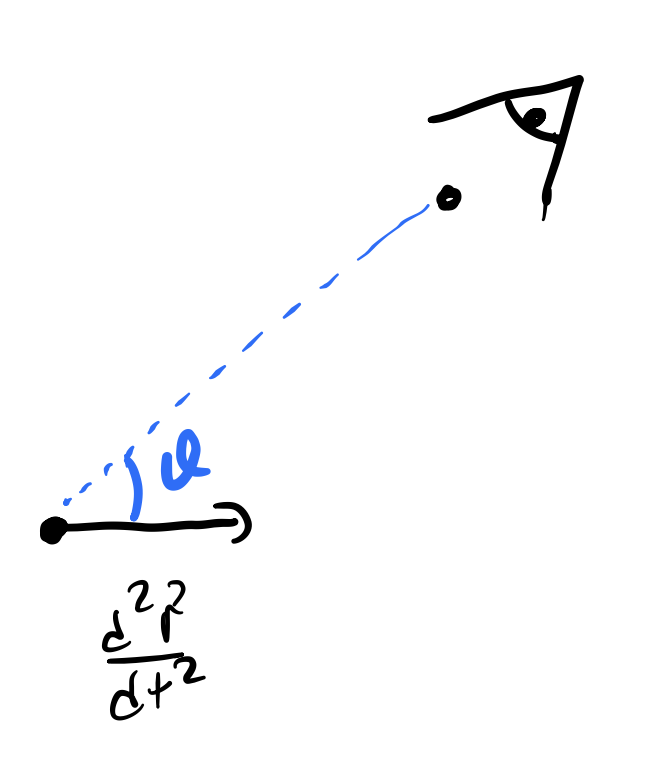
\includegraphics[scale=0.38]{Lectures/Images/lec9-accelangle.png}
\end{center}

It is the same answer as you found for the dipole last quarter:

\begin{equation}
    \dod{P}{\Omega} \propto \sin^2\vartheta
\end{equation}

\subsection{Relativistic Case - Special Limits}
What if we go away from the nonrelativistic limit - therein we consider a velocity:
\begin{equation}
    \dod{\v{r}}{t}(t_{\text{ret}}) = v\zhat
\end{equation}
where $\frac{v}{c}$ is no longer small. Letting $\theta$ be the polar angle

\begin{center}
    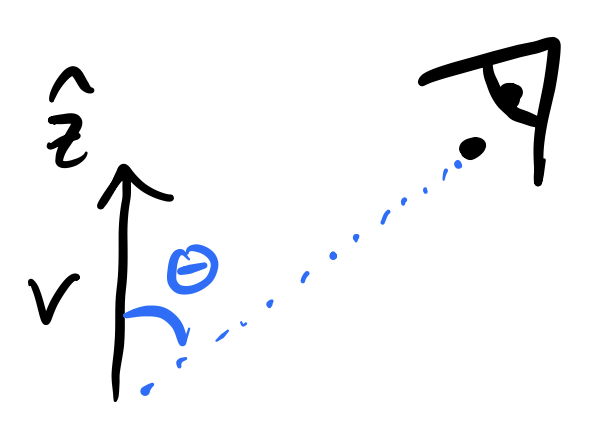
\includegraphics[scale=0.38]{Lectures/Images/lec9-velocangle.png}
\end{center}

We can take:
\begin{equation}
    \alpha = 1 - \frac{v}{c}\cos\theta
\end{equation}

Let us consider two special cases:
\begin{itemize}
    \item $\od[2]{\v{r}}{t}, \od{\v{r}}{t}$ are parallel. This is the case, e.g., in a linear accelerator. In that case we have:
    \begin{equation}
        \left(\dod{P}{\Omega}\right)_{\parallel} = \frac{q^2\mu_0}{16\pi^2 c}\frac{\sin^2\theta}{(1 - \frac{v}{c}\cos\theta)^6}\abs{\dod[2]{\v{r}}{t}}^2
    \end{equation}
    \begin{equation}
        \left(\dod{P'}{\Omega}\right)_{\parallel} = \frac{q^2\mu_0}{16\pi^2 c}\frac{\sin^2\theta}{(1 - \frac{v}{c}\cos\theta)^5}\abs{\dod[2]{\v{r}}{t}}^2
    \end{equation}
    Note that since the acceleration/velocity are perpendicular, $\vartheta = \theta$ and hence the two angles appearing in the above are the same.
    \item  $\od[2]{\v{r}}{t}$ and $\od{\v{r}}{t}$ are perpendicular. This is the case, e.g., when a particle is moving in a circle, where the acceleration points into the center and the velocity points tangent to the circle. In this case, we find:
    \begin{equation}
        \left(\dod{P}{\Omega}\right)_{\perp} = \frac{q^2\mu_0}{16\pi^2 c}\frac{1}{(1-\frac{v}{c}\cos\theta)^2}\abs{\dod[2]{\v{x}}{t}}^2\left[(1 - \frac{v}{c}\cos\theta)^2 - (1 - \frac{v^2}{c^2})\sin^2\theta\cos^2\phi\right]
    \end{equation}
    Where $\theta, \phi$ are the Euler angles (polar and azimuthal angle of the observer relative to the velocity and acceleration... I think).
\end{itemize}

A remark - in the $v \to c$ limit, the power is concentrated in the forwards direction.


\subsection{Larmor Formula and Generalization}
When designing an accelerator, we want to know the total power that gets radiated. This can be calculated by integrating over all solid angles:
\begin{equation}
    P = \int d\Omega \dod{P}{\Omega} = \int \sin\theta d\theta d\phi \dod{P}{\Omega}
\end{equation}
In particular in the limit that $v \ll c$, you saw last quarter (p.84 in Wald) that:
\begin{equation}
    P_0 =  \frac{q^2\mu_0}{6\pi c}\abs{\dod[2]{\v{r}}{t}}^2_{\text{ret}}
\end{equation}
This is an interesting formula, because we can calculate the energy that gets lost over the period of acceleration (assuming the particle does not approach relativistic speeds, for $P_0$). We can analyze the units:
\begin{equation}
    \frac{E}{T} = P = \frac{q^2 \mu_0}{c}\left(\frac{L}{T^2}\right)^2
\end{equation}
from Coloumb we know that:
\begin{equation}
    E = \frac{1}{\e_0}\frac{q^2}{L} = \frac{q^2\mu_0}{c^2}\frac{1}{L}
\end{equation}
and so we find:
\begin{equation}
    c^3 = \frac{L^3}{T^3}
\end{equation}
so the dimensions check out. This is a useful check of your results, e.g. on your midterm if you have time.

To generalize the Larmor formula, we have to consider finite $\frac{v}{c}$. Either we can redo the entire calculation with all the factors of $v$ we neglected. But there is a quicker way; that is to note two things:
\begin{itemize}
    \item $P$ is a Lorentz scalar
    \item $P$ only depends on $\v{v}, \dot{\v{v}}$.
\end{itemize}
The second expression is obvious. The first is a little more subtle, you can see it in Wald 183, but it has to do with the fact that:
\begin{equation}
    P = \dod{E}{t}
\end{equation}
and both $E, t$ are zeroth components of four-vectors. With these two facts, we find that the analog of the total power is:
\begin{equation}
    P = \frac{q^2\mu_0}{6\pi c}\gamma^6\left[\abs{\dot{\v{v}}}^2 - \left(\frac{\v{v} \times \dot{\v{v}}}{c}\right)^2\right]
\end{equation}
Next time, we have 20 minutes more discussion on this topic, and that concludes the midterm coverage.